\chapter{Realisierung}
\label{cha:realisierung}

\section{System-Architektur}
TODO

Die System-Architektur MindSphere ist wie in Skizze ~\ref{fig:MSSystemArchitektur} aufgebaut:

\begin{figure} [H]
\centering
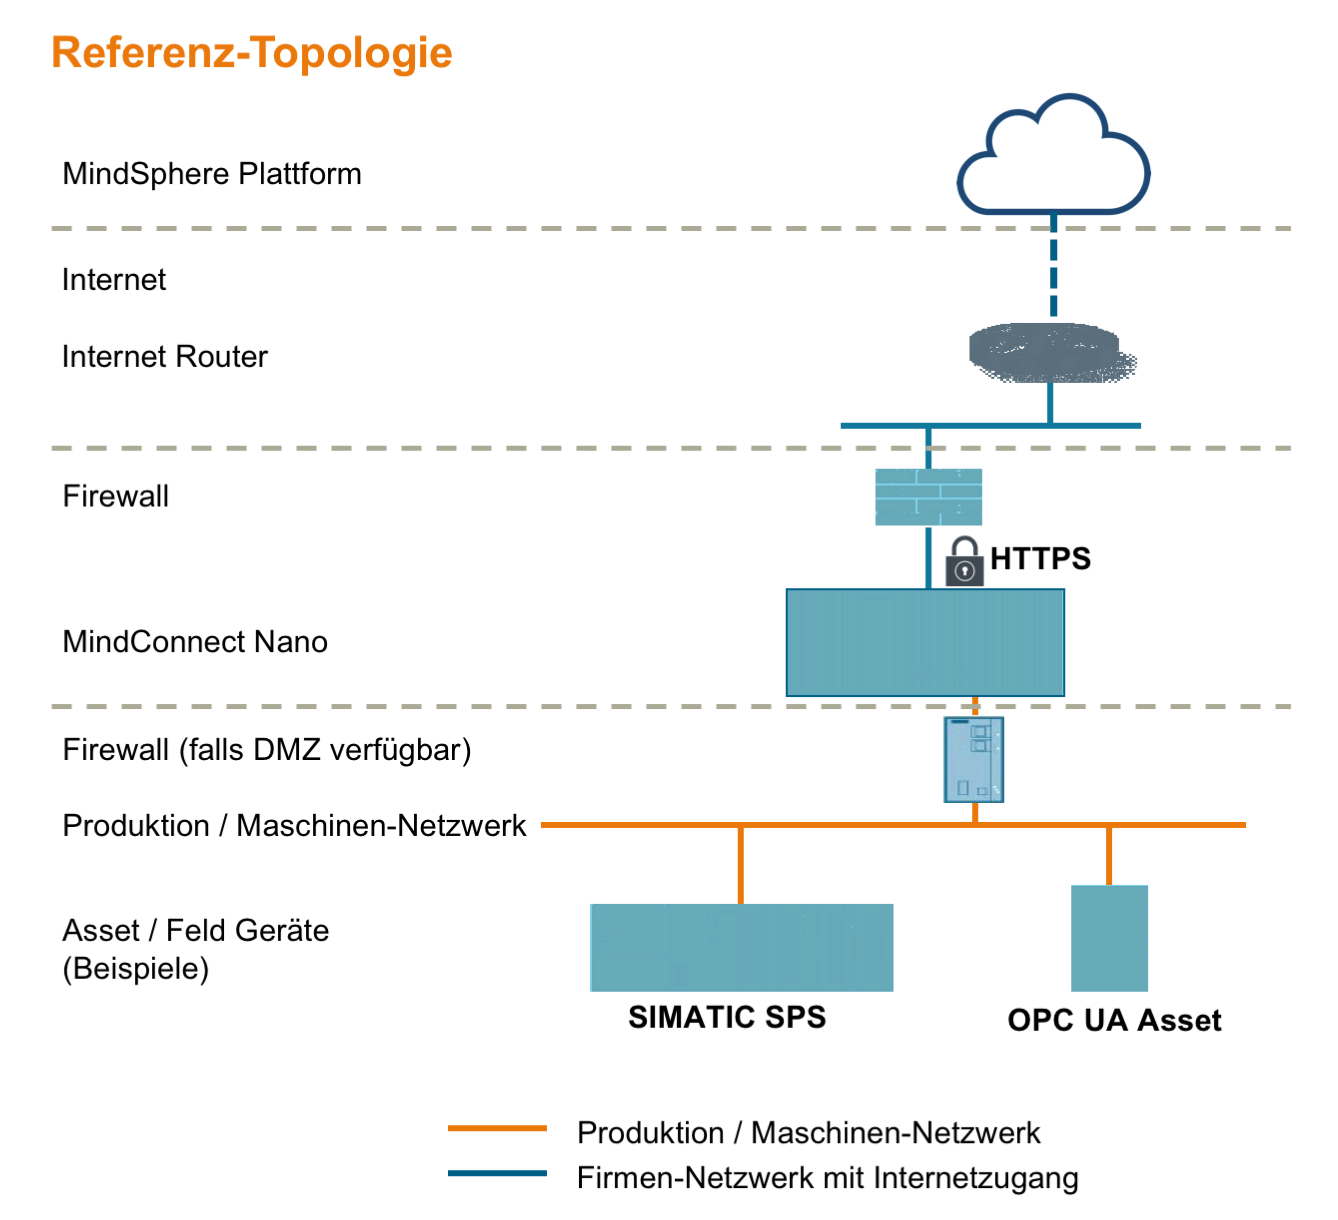
\includegraphics[width=0.8\textwidth]{MSArchitektur.png} 
\caption{Systemskizze der Architektur von MindSphere (vgl. \cite{SiemensMSMCSecurity}).}
\label{fig:MSSystemArchitektur}
\end{figure}

Auf der untersten Ebene im Produktions- bzw. Maschinen-Netzwerk befinden sich die \ac{SPS} mit optional vorgeschaltetem Router, falls das System über eine \ac{DMZ} verfügt. Das integrierte MindConnect Element wird zwischen Maschinen-Netzwerk und Firmen-Netzwerk mit Internetzugang eingebunden. Über eine Firewall und einen Router verbindet sich das MindConnect Element mit der MindSphere-Cloud. Wesentlich ist dabei, dass Daten ausschließlich von den Assets gesammelt und in die Cloud transferiert werden, jedoch der umgekehrte Weg aus Sicherheitsgründen nicht ermöglicht wird.

\subsection{Voraussetzungen für MindSphere}
TODO

\subsection{Arbeiten mit MindSphere}

\subsubsection{Einbinden von MindSphere}
Um MindSphere in ein bestehendes System einzubinden, müssen folgende 3 Schritte durchgeführt werden (siehe Abb.~\ref{fig:MSEinbinden}):

\begin{enumerate}
\item MindSphere Konto anlegen und MindConnect Element integrieren
\item Konfiguration der Datenakquisition
\item System starten
\end{enumerate}

\begin{figure}[H]
\centering
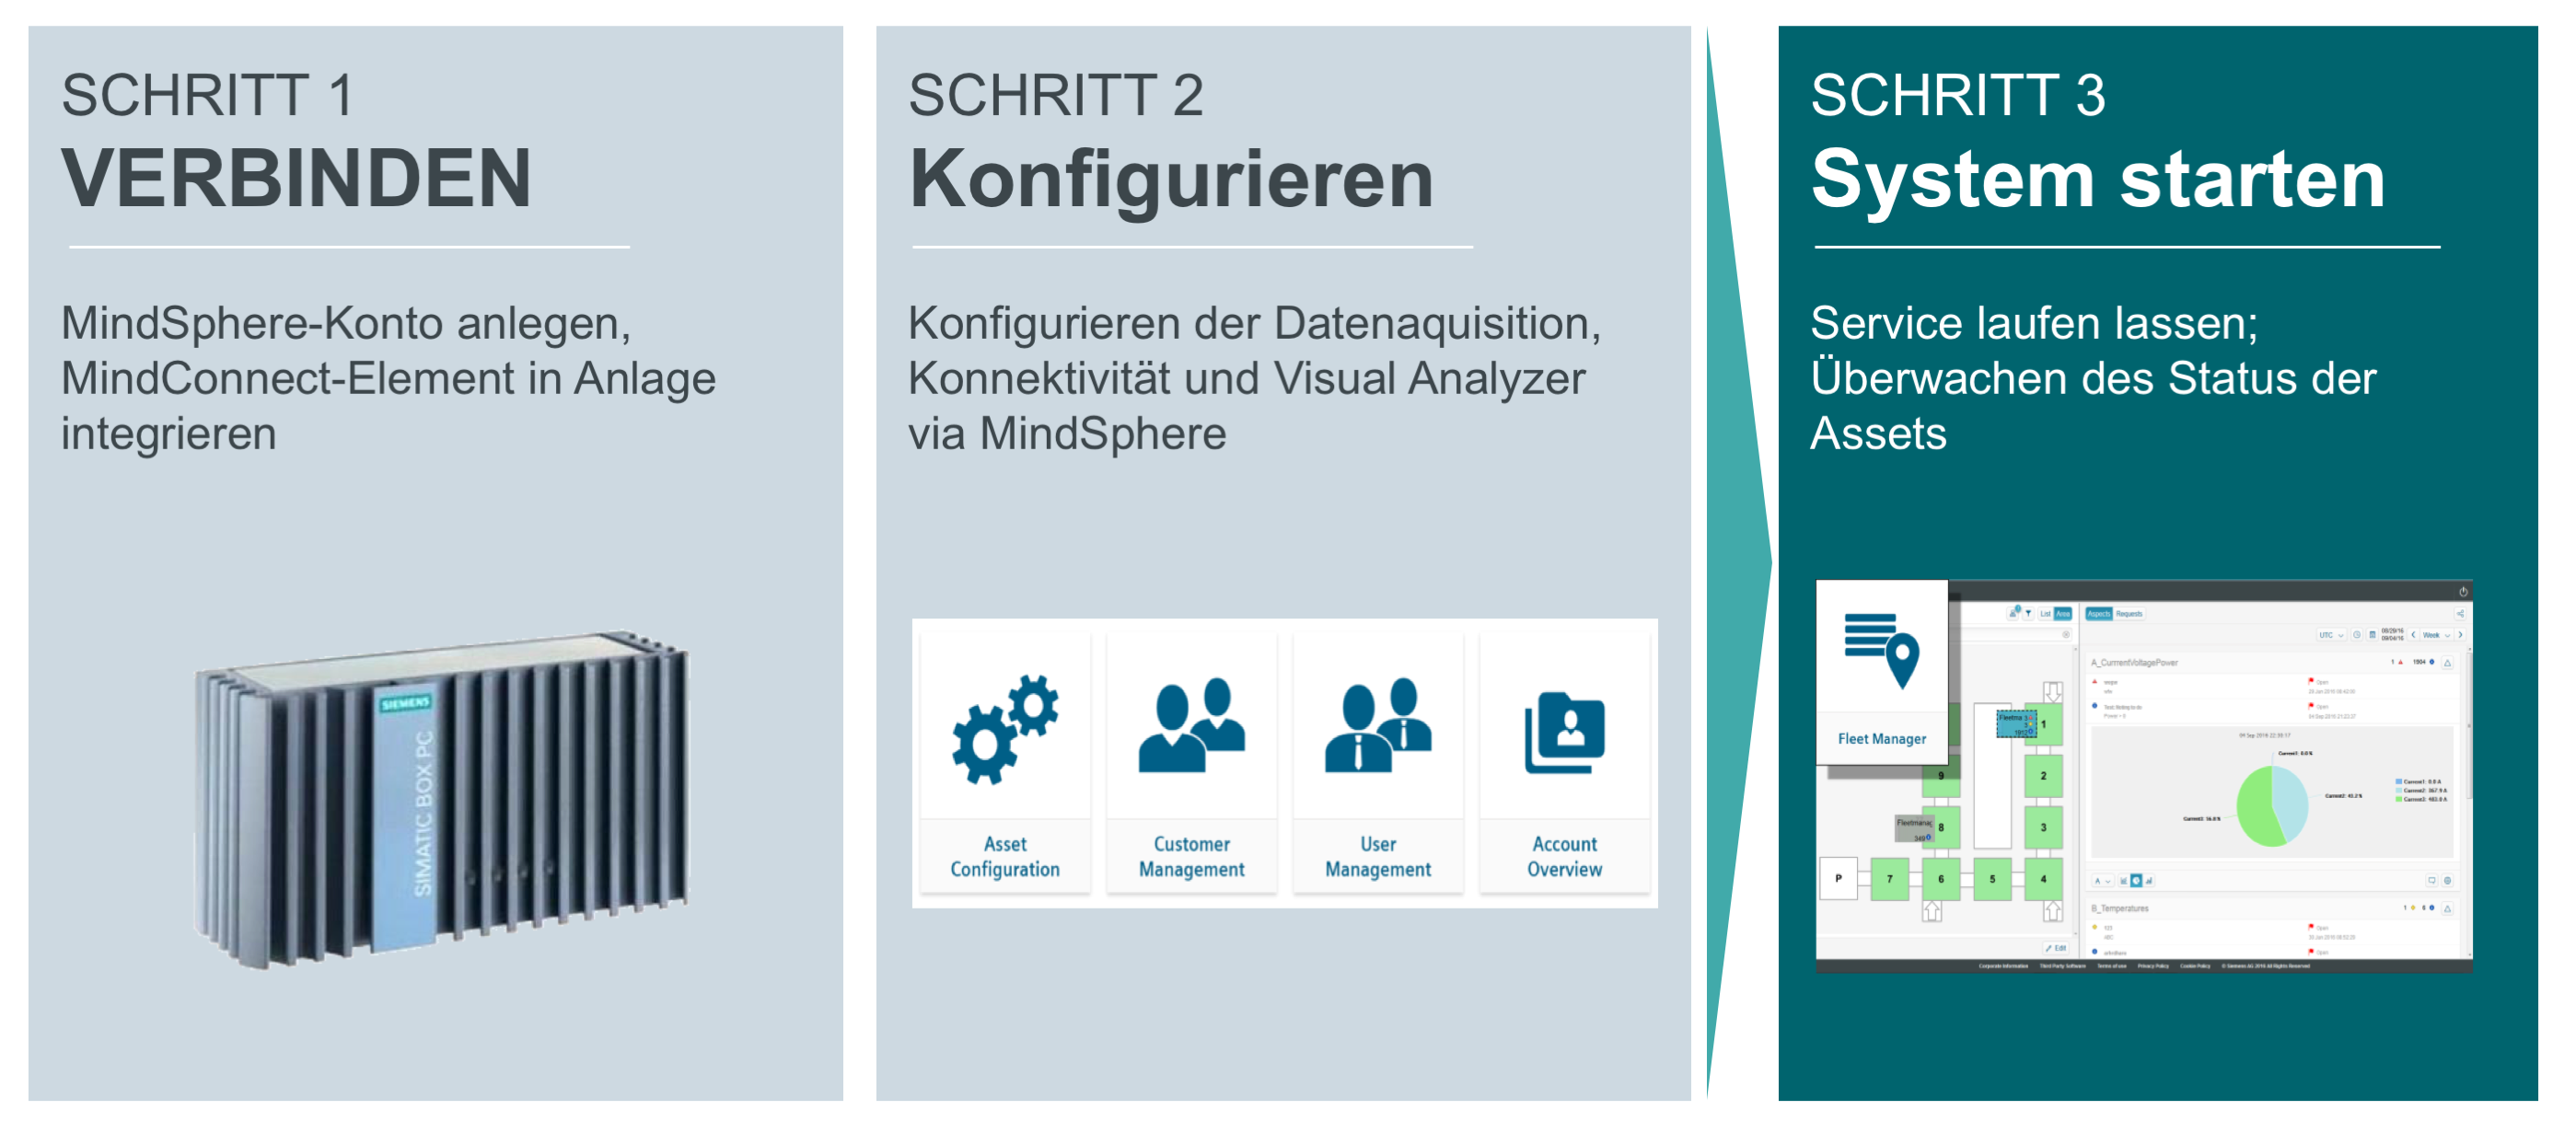
\includegraphics[width=1\textwidth]{MSEinbinden.png} 
\caption{Einbinden von MindSphere in bestehendes System (vgl. \cite{SiemensMSIntroduction}).}
\label{fig:MSEinbinden}
\end{figure}

\textit{Schritt 1}: Als erstes muss ein MindSphere Konto angelegt werden. Dabei gibt es die Unterscheidung zwischen Benutzerkonto (MindAccess User) und Entwicklerkonto (MindAccess Developer). Das Benutzerkonto erlaubt den Zugang zu den eigenen Daten im MindSphere-Ökosystem und die Benutzung der bereit gestellten MindApps. Inkludiert sind dabei zusätzlich 50 Benutzer (Endkunden), welche der MindAccess-Benutzer (Mieter) hinzufügen kann. 

Gegenüber einem Benutzerkonto können mit einem Entwicklerkonto auch Applikationen entwickelt bzw. verändert werden. 

Innerhalb des Entwicklerkontos werden wiederum drei verschiedene Konten angeboten: in den Größen S, M und L.
Eine Gegenüberstellung der Berechtigungen je nach Entwicklerkonto-Größe in Bezug auf Anzahl der EntwicklerInnenlizenzen, Anzahl der BenutzerInnen im Produktionsbereich, dem Test- und Entwicklungsspeicher und dem Speicher für Produktion ist in Tabelle \ref{tab:mindAccessDeveloper} ersichtlich.

\begin{table}[H]
	\caption{Gegenüberstellung der verschiedenen MindAccess Developer Konten (vgl. \cite{SiemensMindAccessDeveloper}).} 		\label{tab:mindAccessDeveloper}
	\centering
	\setlength{\tabcolsep}{5mm} % separator between columns 
	\def\arraystretch{1.25} % vertical stretch factor 
	\begin{tabular}{r|ccc}
 	  % \hline
   		& \emph{Größe S} & \emph{Größe M} & \emph{Größe L} \\
    	\hline
    	%\hline
    	Anzahl der EntwicklerInnen & 5 & 10 &  20\\
    	%\hline
        Anzahl der BenutzerInnen\\im Produktionsbereich & -- & 50 &  100\\
    	%\hline
   	 	Test- und Entwicklungsspeicher (RAM) & 8GB & 16GB   & 32GB \\
    	%\hline
        Speicher für Produktion (RAM) & -- & 16GB   & 32GB \\
    	%\hline
  	\end{tabular}
\end{table}





\textit{Schritt 2}: Die Datenaquisition, Konnektivität und Visual Analyzer werden im MindConnect Element via MindSphere konfiguriert.

\textit{Schritt 3}: Das System wird gestartet und läuft. Die gewünschten Daten werden gesammelt.



% marketplace geplant aber noch nicht realisiert.
% Apps derzeit in Java und Java Script
% Apps laufen in Cloud (Backend
% Derzeit 2 Apps: Fleet Manager und ManageMyMachines




\section{Architektur und Design}
TODO
Software (stat.Klassendiagramm, Ablaufdiagramm)

\section{Ausgewählte Implementierungsaspekte}
TODO


\section{Nicht-funktionale Merkmale}
TODO







